%%%%%%%%%%%%%%%%%%%%%%%%%%%%%%%%%%%%%%%%%%%%%%%%%%%%%%%%%%%%%%%%%%%%%%
%%                           INTRODUCTION
%%%%%%%%%%%%%%%%%%%%%%%%%%%%%%%%%%%%%%%%%%%%%%%%%%%%%%%%%%%%%%%%%%%%%


\pagestyle{plain} % No headers, just page numbers
\pagenumbering{arabic} % Arabic numerals
\setcounter{page}{1}


\chapter{Introduction}
The rapid internet adoption in everyday life and the workplace has presented us with new security challenges. Many users are more active on the internet, giving attackers more opportunities to attack these unsuspecting victims. There are various technical security measures such as firewall, encryption, threat hunting software, and engaging automation to mitigate these challenges. However, studies have shown that the human layer is the weakest link in the security chain \cite{jampen} and attackers usually start by targeting the most vulnerable link before performing other detrimental attacks. These attacks with human interaction are generally known as "Social Engineering Attacks."

Prevalent social engineering attacks such as phishing, pretexting (inventing a scenario to convince victims to divulge information they should not divulge), baiting (promising an item or good to trick the victim), quid pro quo (promising something in exchange for information), and tailgating (someone without the proper authentication follows an authenticated employee into a restricted area) use psychological manipulation to trick users into making security mistakes or giving away sensitive information. This thesis will focus on phishing and different detection techniques through our role-playing gameplay.

\section{What is phishing?}
Phishing is one of the most prevalent social engineering attacks in which attackers target users by contacting them through email, telephone, or text message by posing as a legitimate entity \cite{phishing, apwg} to gain trust. Phishers try to obtain personal (potentially sensitive) data, including login credentials and credit card numbers. They can use this information to create fake accounts, ruin credit, steal money, or identity.

Unfortunately, these attacks are challenging to detect because attackers use the computing infrastructure to trick the victim into doing something while the computing system is working as intended. Due to this, even users with a high-end security system can be victims. An example of such is the infamous case of John Podesta \cite{Podesta}, Hilary Clinton's campaign chairman for the 2016 presidential election. The "googlemail.com" in the domain successfully tricked John Podesta and the Clinton campaign's computer help desk to trust the email (See fig:\ref{fig:Podesta}).


Phishing attacks are constantly evolving with different tricks. For example, Podesta's email shows it was initially generated from "googlemail.com," making it seem like it might be from Google, but it was not true. Attackers can use different spoofing techniques to hide the sender's identity. Another common trick attackers use (also present in Podesta's email) is to confuse the user with links hidden behind some text/button or confuse the user with redirecting links (example: TinyURL). As a result, the displayed text/link might not be the final destination. Podesta's team's failure to deal with this phishing email led to leaks of more than 11,000 emails which included private conversations with 2016 presidential nominee Hillary Clinton \cite{anderson_2016}.

\begin{figure}[ht]
    \centering
    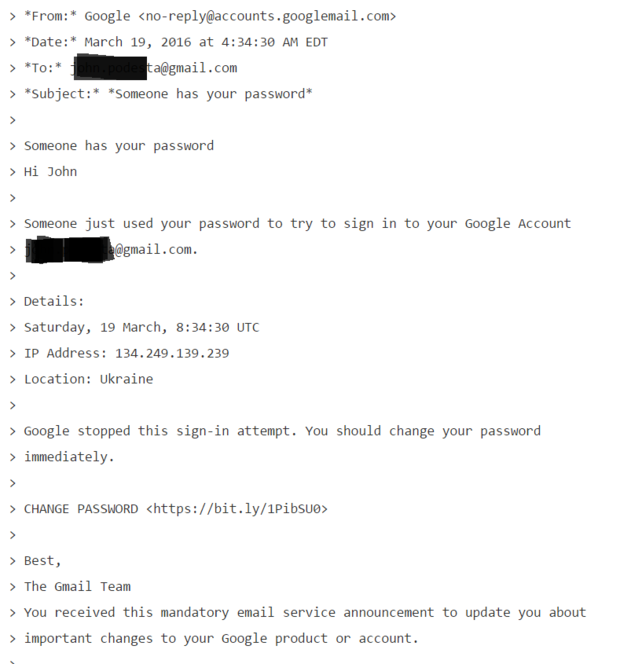
\includegraphics[scale=0.7]{{./section1/podesta.png}}
    \caption[Phishing email sent to John Podesta]{Phishing email sent to John Podesta}
    \label{fig:Podesta}
\end{figure}

Successful phishing attacks are expensive to organizations. In 2020 alone, phishing attacks cost US businesses more than \$1.8 billion, up from \$1.7 billion in 2019 \cite{vade}. These attacks can lead to credential/account compromise, giving the attacker access to sensitive information, et cetera. Attackers may try to use these data for extortion. For example: In 2014, an attack was successful on an invasion of celebrity iCloud accounts, leading to the leaking of nude photos. The leak was initially considered due to a breach on Apple services, but it was a phishing attack. The attackers pretended to be Apple and Google and asked users to change their password \cite{duke_2014, guardian_2014}.

Phishing attacks are continuously rising and have doubled since early 2020. In July 2021 alone, the Anti-Phishing Working Group (APWG), an international consortium that attempts to eliminate fraud and identity theft caused by phishing, saw 260,642 phishing attacks \cite{apwg}. Additionally, Proofpoint, a security enterprise that provides cybersecurity products relating to emails and digital information, found that more than 75\% of organizations faced phishing attacks in 2021 \cite{proofpoint}. These uprising trends in phishing attacks have shown some serious need for mitigations.

\section{Current Mitigations}
The prevention of phishing attacks can be divided into three steps \cite{vayansky}—the first step is preventing the attack from reaching the end-user. We have seen multiple studies on phishing prevention with the help of the machine learning models \cite{yang_zheng_wu_wu_wang_2021, sahingoz_buber_demir_diri_2019}. Machine learning approaches such as K-nearest, XGBoost, CNN, RCNN, Random forest, et cetera. are commonly used to detect patterns and generalize phishing attacks. Some of the models have shown promises with more than 90\% accuracy—however, a study conducted by What.Hack has shown that only one of the ten anti-phishing tools tested could correctly identify over 90\% of phishing websites. That tool also incorrectly identified 42\% of legitimate websites as fraudulent \cite{what_hack}. Moreover, attackers are always looking for the best way to bypass these automated systems and develop new techniques. The evolving nature of phishing attacks calls for an additional layer of security on top of the prevention layer.

If the attacks reach the user, the next step to secure the user is by warning them. Most modern web browsers and email clients warn users of any suspicious activities they detect. For example, the browser actively warns users with pop up for probable phishing sites. In addition, browsers provide passive hints to understand URLs better. Browsers use different shades of white to inform the user about a "fully qualified domain name (FQDN)" (also called absolute domain name), the complete domain name for a specific host on the internet. Figure \ref*{fig:browser_cues} shows a use case for such a hint. Attackers will intentionally have a confusing link to trick users into clicking the link. For example, although "help.google.com.bubble.com/changepassword" seems like an email from Google, the actual domain is bubble.com. The domain owner can add any subdomain to domains they own, such as help.google.com.bubble.com, which can potentially be used in phishing attacks. Modern email clients provide similar hints for spam emails and notify the users if they can not verify the sender. Active warnings are more effective than passive signs \cite{vayansky}. Still, attackers can easily bypass these warnings by creating new sites and context-aware websites or emails every time they are flagged.

\begin{figure}[h]
    \centering
    
\includegraphics[scale=0.7]{{./section1/browser_cues.png}}
    \caption[Browser cues on links]{Browsers uses different shades to indicate the primary link.}
    \label{fig:browser_cues}
\end{figure}

The final step to avoid phishing emails is user training. A study done by Proofpoint shows that 34\% of US respondents believe emails with familiar logos are safe \cite{proofpoint}. The study indicates a general lack of awareness about phishing campaigns among the general population. As emails are the most frequent phishing attacks, many phishing training focuses on training users to detect phishing emails. Our gameplay will focus on emails to train the users against phishing attacks.

One of the most common tools to train users is cyber security videos and reading materials. However,  Kumaraguru et al. saw that users seldom seek these materials and tend to ignore emails directing them to these materials \cite{johnny_phishing}. In addition, they noticed that most users do not spend much time reading security-related tutorials. This calls for an interactive training program to keep the user focused and engaged during training.

We have seen new and existing training materials incorporating gaming techniques. Gamification has been gaining rapid popularity over the past decade\cite{schultz_2021}. It increases engagement by incentivizing learners to pay attention and complete activities. We can observe existing training videos incorporating gaming techniques, such as letting users choose the correct option in the middle of training videos (a mini quiz game) and giving badges after completion. Newer training videos take gamification further and let learners play through various scenarios, make choices and see the rewards or consequences of their decision. For example, "Infosec's Choose Your Own Adventure Security Awareness" Game\cite{infosec_2022} has interactive storytelling to keep the user focused till the end of the video.

Gamification has improved the interactivity with the user, but existing training videos fail to cover the technical details that are commonly found in phishing emails. Our gameplay covers various technical aspects commonly found in phishing emails, such as domains, spoofing, and link hiding techniques attackers use to trick users.

\section{Litearature Review}

\subsection{Serious games}
Gaming approaches in education have been used for over a decade\cite{almeida_2012}. There is a dedicated genre of games (typically online applications), termed serious games. These games communicate specific information that helps introduce relevant concepts and apply those concepts to solve problems. The primary purpose of these games is to promote learning alongside entertainment. With the help of different game design techniques (rewards, story progression, feedback systems), users are more engaged and immersed while learning. In addition, the virtual world also provides users with a safe space to experiment without real-life consequences.

Serious games are used in many fields such as education, healthcare, and training. For example, "Garfield's Count Me In" \cite{count_me_in} helps children in (special education) primary school practice their arithmetic skills. This math game contains different exercises or 'brick,' which form the foundation for a new layer of exercises. The game design help students master the first layer of exercises before moving to the next layer (basic to advanced).

"Killer Flu" \cite{killer_flu} (one of many games by "Persuasive Games") is another example of a serious game that attempts to explain how flu mutates and spreads and how challenging it can be for a deadly strain to affect a large population geographically. The game helps spread awareness by making the player take the role of the flu itself, trying to mutate and then spread it in various conditions. Serious games (such as Killer Flu) can place the user as any character in the game to get the idea across. We use a similar concept in our game by placing the player as the attacker (rather than the victim as many existing training materials do.)


\begin{figure}[h]
    \centering
    \begin{minipage}{0.49\textwidth}
        \centering
        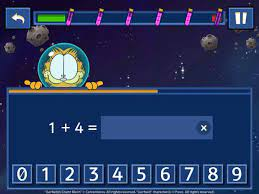
\includegraphics[width=0.9\textwidth]{./section1/garfield.jpeg}
        \caption{Garfield's Count Me In}
    \end{minipage} \hfill
    \begin{minipage}{0.49\textwidth}
        \centering
        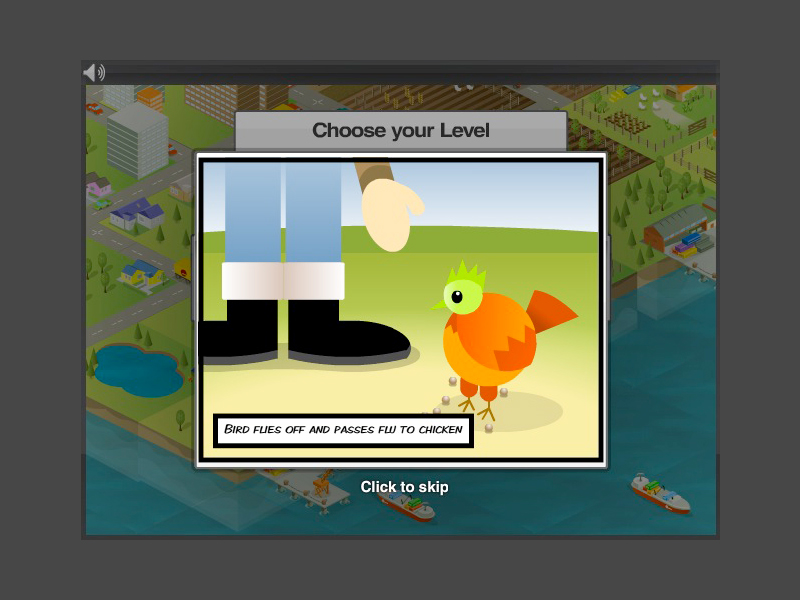
\includegraphics[width=0.9\textwidth]{./section1/killer_flu.jpg}
        \caption{Killer Flu}
    \end{minipage} \hfill
\end{figure}

There have been various studies about using games as a practical phishing training module. Hendrix et al. \cite{hendrix_al_sherbaz_bloom_2016} compared the effectiveness of cyber security training tools with some popular games designed for cyber security training. They found that existing games, in general, had a positive impact on learning, with positive education experience.

We can broadly classify current training games into three main categories. We discuss each of these categories and provide some examples of each type in the following sections.

\subsection{Board and card games}
There have been studies based on non-computer-based games. For example, Control-Alt-Hack \cite{control_alt_hack} and "smells phishy" \cite{smels_phishy} are card games aimed to train users against phishing. Both the games show promise in their approaches and teach the user what to be aware of (such as spelling mistakes, phishing links) through their gameplay. After playing the game, users reported higher efficiency and ability to detect phishing emails.

Although both the games show promise in their approach, non-computer-based games have some inherent limitations. The games have a barrier of entry as it requires pre-setup (with the need for the cards and boards). Furthermore, once the games are deployed, they are permanent, limiting their ability to train and evolve against new phishing attacks. Finally, board and card games fail to communicate the context of the attack and lack examples of where they might be used. For example, although the game might have a "hiding links" card, the users lack knowledge on how and when it might be used. The limited skills these games provide may not be best suited as an individual training module.

\subsection{Phishing Link (URL) training}
There have been numerous computer games about phishing. However, many studies focus on one common category: training users to verify phishing links. Anti-Phishing Phil \cite{anti_phishing_phil} is one of the pioneers in this field. Their gameplay puts the user as a fish. The goal of the fish is to grow larger by eating the good bugs (non-phishing links) and avoiding the bait (phishing links). The game has four different levels, with each round focusing on another type of deceptive URL. Players move to the next level after correctly identifying six out of eight URLs.

There are other similar games to Anti-Phishing Phil. For example, Phish Phinder \cite{phish_phinder} builds upon the Anti-Phishing Phil storyline and game design. However, it differentiates itself from Anti-Phishing Phil by integrating self-efficacy in the game design to enhance phishing avoidance motivation and behavior among users. They were able to positively impact self-efficacy by adding conceptual knowledge (through challenges) and procedural knowledge (through increasing levels and repetition of conceptual knowledge).

"Building Confidence not to be Phished"\cite{gamified_approach} by Baral et al. developed a game prototype aimed to enhance an individual's self-efficacy in phishing threat avoidance. They developed a ballon shooter game where the main character has to shoot balloons with legitimate URLs (similar to previous games). Although the links and hints are displayed in a different context, this game tries to achieve the same goal as previous games.

All these games have one thing in common: they teach users how to identify legitimate URLs through their gameplay. As URLs are one of the most critical factors while detecting phishing emails, gameplay dedicated to recognizing phishing URLs serves as a suitable training module. Anti-Phishing Phil results show that their game has a good impact compared to existing training material to differentiate legitimate links from phishing links.

However, these games might not be suitable as standalone training against phishing. Although URL training games are a sound training module, these games fail to train users on some common tricks seen in phishing attacks. For example, one of the most significant limitations of these games is the lack of context on where the link might appear. As such, attackers can use different link hiding techniques to trick the user into clicking the link. Moreover, attackers use psychological manipulation to trick users into clicking the link by creating a sense of urgency, fake giveaways, or making it seem like an email from somebody individuals know to trick people into clicking the link.

\subsection{Role playing game}
"What.Hack" \cite{what_hack} saw the shortcomings of the link-based game and developed gameplay that train the user on links as well as email context. It puts the user as a bank employee required to process emails to acquire contracts and protect their network from cybercriminals. The game approaches the training by having the user role play as a victim and looking at different techniques found in actual attacks. The game's goal is to block phishing attempts and allow legitimate emails. It simulates the harmful effects of phishing by "firing" the employee in-game if they allow too many phishing emails, take too long, or misclassify a significant number of legitimate emails as phishing emails.

\begin{figure}[h]
    \centering
    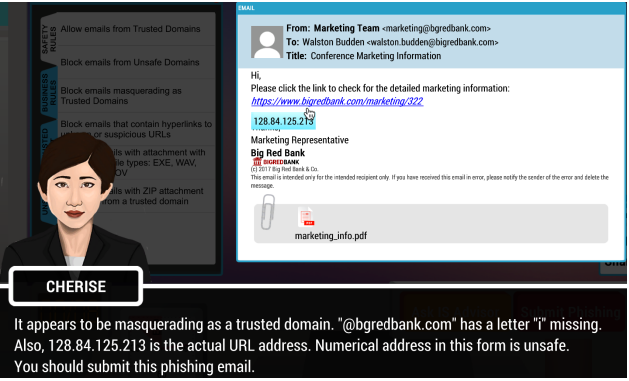
\includegraphics[width=0.9\textwidth]{./section1/what_hack.png}
    \caption{What.Hack gameplay}
\end{figure}

"What.Hack" gameplay incorporates previous studies' different techniques and builds upon them. In addition, its context-based email training module solves one of the drawbacks of link-based training games. Since players are looking at full emails (both phishing and legitimate) obtained from the real world, users can better recognize the context of the email and what to look out for in emails to stay protected. Moreover, the emails generated in this game successfully incorporate the objective of primary link-based game goals.

The result from "What.Hack" shows clear improvement regarding link-based games. In comparison to Anti-Phishing Phil, "What.Hack" improved players correctness in identifying phishing emails by 36.7\% \cite{what_hack}.

\section{Objective}

"What.Hack" clearly demonstrated that role-playing games with contextual emails were more effective than existing gameplays. Unfortunately, we could not find any other significant study that tried to build upon this finding. Therefore, we have developed gameplay inspired by "What.Hack" but approached the role-playing aspect as an attacker instead of a victim.

Current phishing training programs focus on training the user as a victim. Our game tries to approach training from a new direction by placing the player as an attacker. This approach will let the users see what the phisher might concentrate on while creating a phishing email and, in turn, use that knowledge to detect phishing emails. The training objective of our game is similar to exisiting games and tries to build upon it. Table \ref{tab:game-type} compares the main training objective of our game with existing games.

\begin{table}[!ht]
    \resizebox{\textwidth}{!}{%
        \addtolength{\tabcolsep}{-10pt}
        \begin{tabular}{p{0.13\textwidth} p{0.48\textwidth} l l l}
            \hline
            \textbf{Game Type}   & \textbf{Description}                                                                                 & \textbf{URL}          & \textbf{Spear} & \textbf{Spoof} \\
            \hline
            \textbf{Link Based } & Teach users to differentiate phishing links from non-phishing links                                  & \centering \checkmark &                &                \\

            \textbf{Board Game}  & Teach users high- level security concepts                                                            & \checkmark            & \checkmark     & \checkmark     \\
            \textbf{What.Hack}   & Teach players to defend against phishing attempts in realistic simulation game (playing as a victim) & \checkmark            & \checkmark     &                \\
            \textbf{Our Game}    & Teach players to recognize and defend against phishing attempts by role playinig as a victim         & \checkmark            & \checkmark     & \checkmark     \\
            \hline
        \end{tabular}%
        \addtolength{\tabcolsep}{10pt}
    }

    \caption{Different type of training games and their main objectives}
    \label{tab:game-type}
\end{table}

Our goals for the study can be summarized as:

\begin{itemize}
    \item We designed and developed a phishing training game that attempts to incorporate the objectives of the current existing games and build upon them. Our game includes link hiding training and provides context to those links.
    \item We compare the participants' performance before and after playing the game. We evaluate users' results and try to understand user thought processes behind each decision.
    \item Finally, we list some of the insights found during the survey and list potential mitigation and training.
\end{itemize}



